% ==============================================================================
%
%                             Mission
%
% ==============================================================================
\chapter{Mission} \label{chapt:mission}
The following sections will first cover the starting point based on appendix \ref{app:aufgabenstellung} and the available resources (appendix \ref{app:technicial_requirements}). Different possible solutions will be covered in \ref{chapt:solutions} before presenting the concept in \ref{chapt:mission:concept}. \\

In a world of self driving cars and virtual reality, having a digital copy of
the real world yields several benefits. Cars can be trained in a virtual city
to increase the performance of their algorithms and video games could get more
realistic if the player could walk through the streets of a major city. Gathering this data is one problem and processing the images is another. Pictures have to be converted, analyzed and processed. This requires a great deal of computational power for a task that is repeated several times.

% ==============================================================================
%
%                             Starting Point
%
% ==============================================================================
\section{Starting Point}
To accelerate intense image processing a dedicated hardware approach is investigated. To do so, a basic image processing algorithm such as the Wallis filter is implemented in an FPGA that communicates over a network with a host computer. The image processing task should later be distributed onto multiple FPGAs to accelerate the processing even more \cite{nomokoReqs}. Before listing possible solutions the available resources need to be dissected.

\subsection{FPGA Board} \label{chapt:mission:fpgaboard}
\begin{figure}[tb!]
    \centering
    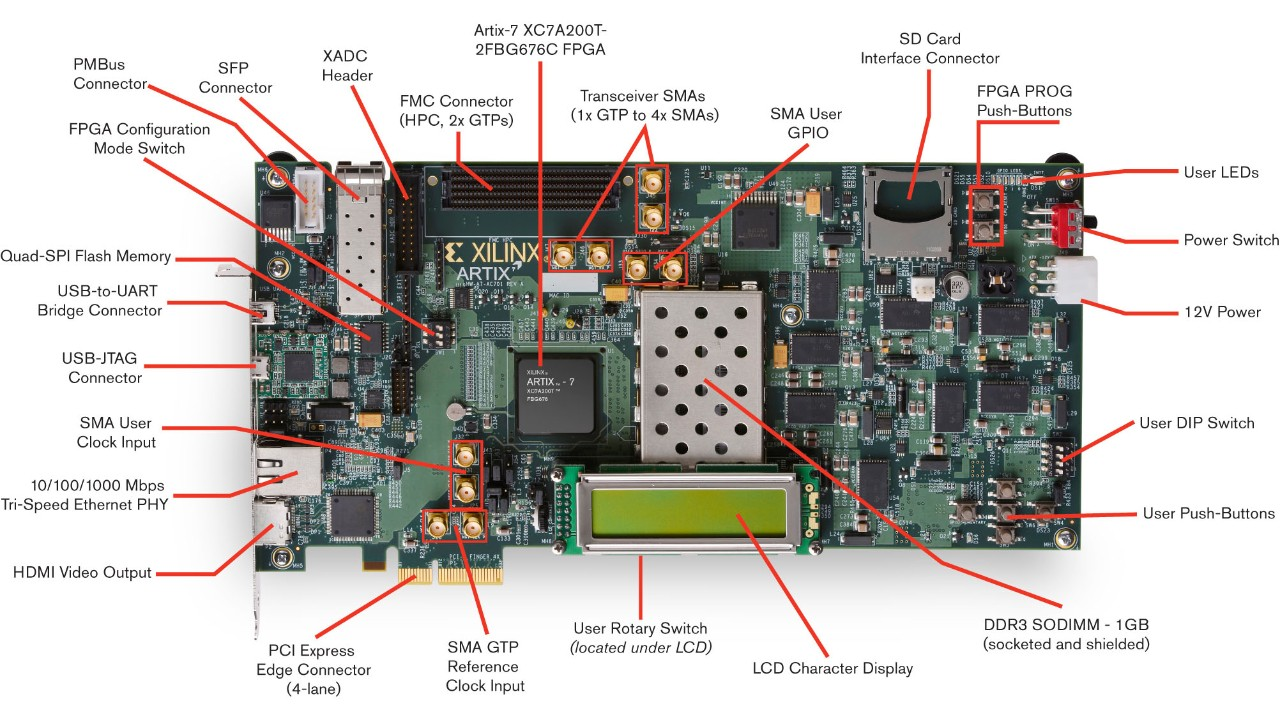
\includegraphics[width=\textwidth]{images/mission/ac701.png}
    \caption{Xilinx AC701 Evaluation Kit \cite{image_ac701}}
    \label{fig:ac701}
\end{figure}

The Xilinx AC701 Evaluation Kit is used as development platform. It features an
Artix-7 FPGA and several useful on-board peripherals. The JTAG interface is used
for configuration and debugging of the FPGA. To connect the platform to the
network, a Gigabit Ethernet PHY handles the first layer of the OSI model in
hardware (see chapter \ref{chapt:theory:physical}). Storing data is possible in the DDR3 memory
module. Table \ref{tab:ac701} shows a summary of the important peripherals on
the AC701 board.
\\
\begin{table}[b!]
    \centering
    \begin{tabular}{l l}
        \toprule
        Part & Description \\
        \midrule
        FPGA & XC7A200T-2FBG676C \\
        JTAG & Onboard JTAG configuration circuitry to enable configuration over USB \\
        Memory & DDR3 SODIMM 1GB up to 533MHz / 1066Mbps \\
        Ethernet & 10/100/1000 Mbps Ethernet (RGMII) \\
        \bottomrule
    \end{tabular}
    \caption{Xilinx AC701 key board features \cite{xilinx_ac701}}
    \label{tab:ac701}
\end{table}

The XC7A200T FPGA is part of the Artix-7 family. It is optimized for high logic
throughput at low costs. Important for this project is the number of logic cells
and the amount of on-chip memory. With more logic cells available, data can be
processed parallel and the throughput increases. Processing more data at the
same time also requires the data to be stored. Therefore on-chip memory, also
called block memory, is used to have fast access to the data. Table 
\ref{tab:XC7A200T} lists the relevant numbers of resources.

\begin{table}[tb!]
    \centering
    \begin{tabular}{l l}
        \toprule
         & XC7A200T \\
        \midrule
        Logic Cells & 215k \\
        DSP Slices & 740 \\
        Block Memory & 1642 KB \\
        \bottomrule
    \end{tabular}
    \caption{XC7A200T key features \cite{xilinx_ac701}}
    \label{tab:XC7A200T}
\end{table}


\subsection{Communication} \label{chapt:mission:communication} 
In the preceding project \cite{p5report} a Ethernet communcation between PC and
FPGA was established. This included a UDP based protocol that was implemented on
the PC and on the FPGA in form of an IP core. Basic file transfers are working
but many features such as reliable transfer using acknowledge and retransmission
exist only on paper. The work in this project is built
upon the IP core from project 5 while improvements and modifications are made to
the IP core.

\begin{figure}[tb!]
    \centering
    % 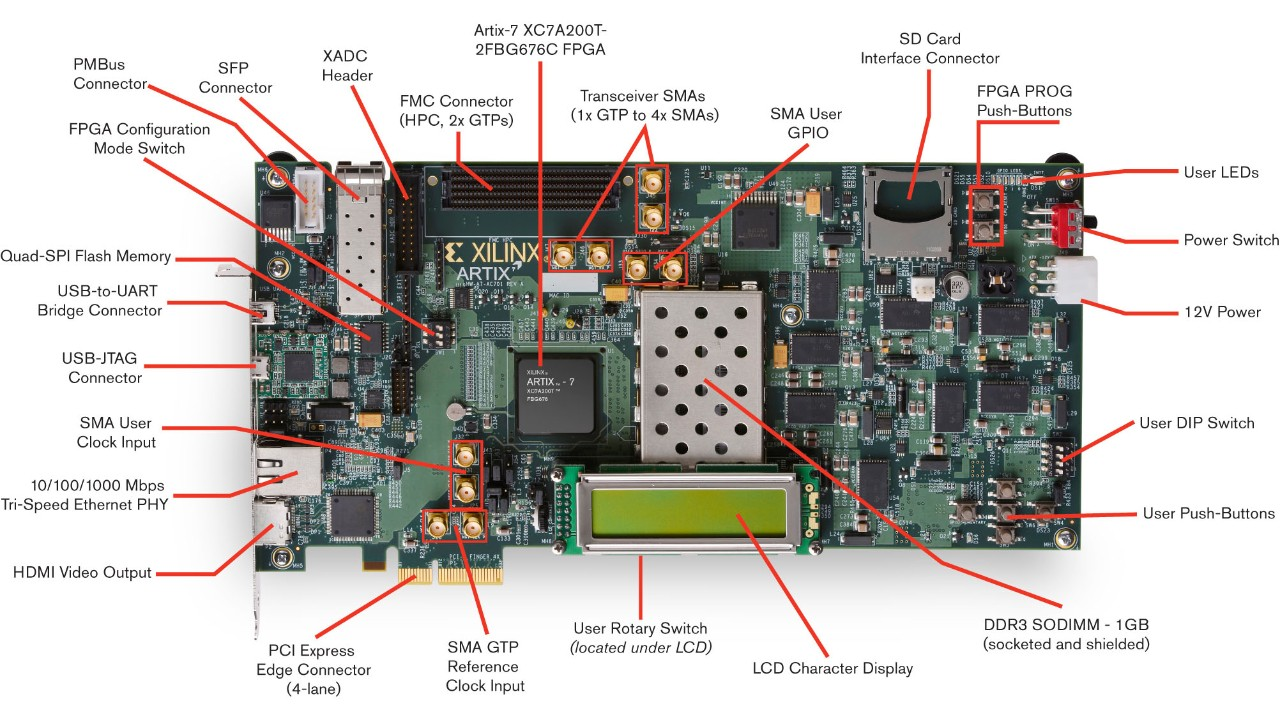
\includegraphics[width=\textwidth]{images/mission/ac701.png}
    \caption{UFT IP core from project 5 \cite{p5report}}
    \label{fig:uftipcorep5}
\end{figure}

\todo[inline]{figure p5 UFT ip core from block design}

\subsection{Image Size}
The customer Nomoko has a camera with a resolution of 1500MPixel (\ref{app:technicial_requirements}). If this is a color image with 24 bit RGB values, the following file size will result:
\begin{equation}
    File Size = Pixel_{tot} * Pixel_{size} = 1500MPixel * 24bit = 36Gbit \cong 4.4GByte
    \label{eq:filesize}
\end{equation}

\subsection{Wallis Filter} \label{chapt:mission:wallis}
The employer, Nomoko, wants the Wallis filter to be implemented. The Wallis filter is used for local contrast enhancement. For example, the filter can compensate the house shadows in images and get more details from the image. 
The Wallis filter is based on the equation \ref{eq:wallis_filter} as explained in chapter \ref{ch:th_wallis_filter}.


\subsection{Development Environment}
The image processing algorithm is written in Vivado HLS (\ref{app:technicial_requirements}). With Vivado HLS, an IP core for the Vivado HLx can be generated from a C/C++ code. Vivado HLS is useful when programming algorithms and afterwards translating them into hardware description language. \\ 
\\
Communication is implemented with configurable IP blocks provided by Xilinx or third party providers. Vivado HLS is mainly used for the dataflow in the FPGA (\ref{app:technicial_requirements}).

% ==============================================================================
%
%                             Possible Solutions
%
% ==============================================================================
\section{Possible Solutions} \label{chapt:solutions}

\subsection{Image Processing} \label{chapt:mission:ip}
The Wallis algorithm is based on the neighborhood operation (\ref{ch:th_wallis_filter}). Therefore, the borders of the image must be considered separately (\ref{ch:th:neighborhood}). There are three possible solutions to the border problem:

\begin{itemize}
\item The border pixels are not considered. This means that the destination image will be smaller depending on the size of the neighborhood
\item The pixels required outside the image are extrapolated according to the closest pixels
\item The image is continued periodically
\end{itemize}

\subsection{Dataflow} \label{chapt:mission:dataflow}
As described in \ref{ch:th_wallis_filter} the Wallis filter requires a
neighbourhood of pixels to do its calculations. Therefore the data comming from
the communication part must be buffered and fed to the Wallis filter in a given
order. Further details are described in chapter \ref{chapt:dataflow}. Following
realisations may be considered for the control of the dataflow:\\

\textbf{Data preparation on PC:} The image data is prepared on the PC and sent
in the right order. This method is simple to realise and requires no
additional FPGA ressources. On the other hand, data may be sent more than once
which results in a decrease of throughput.\\

\textbf{Soft microprocessor core:} Image data is sent to the FPGA and stored in
FPGA memory. A microcontroller implemented in FPGA logic then dissects the data
and feeds it to the Wallis filter in the right order. Hence the data is buffered
the Ethernet throughtput can reach its maximum. The downside to this solution
is that such a soft microprocessor core may take more FPGA ressources than a
dedicated approach.\\

\textbf{Controller IP-core:} An IP core is developed that handles the specific
task of managing the dataflow between the communication and Wallis cores. This
approach takes little FPGA ressources but involves more time to develop.

\subsection{Scalability} \label{chapt:mission:scalability}

% ==============================================================================
%
%                             Concept
%
% ==============================================================================
\clearpage
\section{Concept} \label{chapt:mission:concept}
Now that the possible solutions for dataflow, image processing and scalability
are dissected, the way of proceeding can be concluded.\\


\textbf{Scalability}
    \begin{itemize}
        \item Use stream interfaces where possible
    \end{itemize}

\textbf{Image processing}
    \begin{itemize}
        \item The border pixels are not considered for simplicity. The destination image will be smaller than the source image.
        \item The image is sent in several parts to the FPGA. Since 4.4GByte (see equation \ref{eq:filesize}) do not have space on the FPGA (see chapter \ref{chapt:mission:fpgaboard}).
    \end{itemize}

\textbf{Dataflow}
    \begin{itemize}
        \item Extend the communication with acknowledge and retransmission
        \item Realize a controller IP-core to handle the dataflow between
        communication and Wallis filter
    \end{itemize}

Figure \ref{fig:blockdiagram} shows the top level block diagram. Image data is
sent from the PC to the FPGA over Ethernet. The communication block handles the
file transfer and stores the image data in FPGA block memory. A controller core
then feeds the data in the right order to the Wallis filter and stores the
results again in block memory. The controller sends a command to the
communication cores which then starts sending the processed image data back to
the PC.

\begin{figure}[b!]
    \centering
    % % \tikzsetnextfilename{system-overview}
\begin{tikzpicture}[
    rounded corners=0mm,
]
    %coordinates
    \coordinate (corig)      at (0,0);
    \coordinate (cmonitor)   at (0,0);
    \coordinate (ccom)       at (5,0);
    \coordinate (cip)        at (10,0);


    %nodes

    \begin{pgfonlayer}{main}
        \node[draw, fill=white, minimum width=3.2cm, minimum height=1.8cm, anchor=west, align=center, rounded corners=1mm] (mon) at (cmonitor) {};

        \node[draw, fill=white, minimum width=2.1cm, minimum height=0.4cm, anchor=west, align=center, rounded corners=2mm, below=0.2cm of mon] (stand) {};
        \node[draw, fill=white, minimum width=0.2cm, minimum height=0.1cm, anchor=south, align=center] (stange) at ($(stand.90) + (0,-0.04)$) {};



        \node[draw, fill=white, minimum width=3cm, minimum height=1cm, anchor=west, text width=2.8cm, align=center, right = 2cm of mon] (com) at (ccom) {Communication};
        \node[draw, fill=white, minimum width=3cm, minimum height=1cm, anchor=west, text width=2.8cm, align=center, right = 1cm of com] (mem)  {Memory};
        \node[draw, fill=white, minimum width=3cm, minimum height=1cm, anchor=west, text width=2.8cm, align=center, below = 1cm of mem] (control)  {Controller};

        \node[draw, fill=white, minimum width=3cm, minimum height=1cm, anchor=west, text width=2.8cm, align=center, left = 1cm of control] (ip) {Image\\Processing};
        

        \node[inner sep=0pt, anchor=west] (whitehead) at ($(cmonitor) + (0.1,0)$)
            {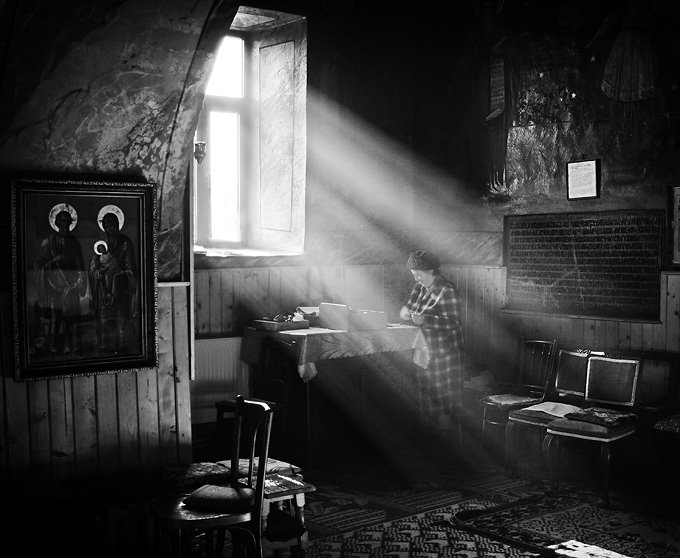
\includegraphics[width=1.4cm]{images/mission/room.png}};
        \node[inner sep=0pt, anchor=west] (whitehead) at ($(cmonitor) + (1.7,0)$)
            {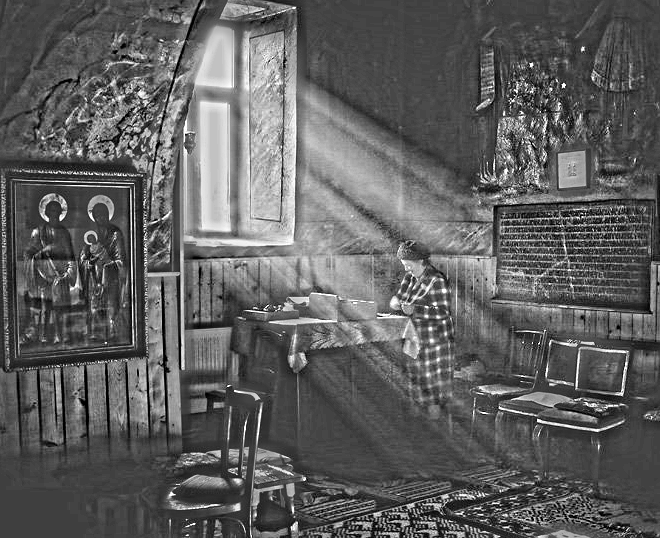
\includegraphics[width=1.4cm]{images/mission/room_fpga_vhdl_v20.png}};

        \node[] (eth) at ($(cmonitor) + (4.5, 1.0)$) {LAN};
        
        \draw[line width = 0.5mm] ($(eth) + (0,-1.0)$) ellipse (0.2cm and 0.5cm);
    \end{pgfonlayer}

    % FPGA box
    \begin{pgfonlayer}{main}
        \node[above = 0.2cm of com, xshift=-1.5cm] (fpga) { FPGA };
    \end{pgfonlayer}
    \begin{pgfonlayer}{foreground}
        \node (f_fpga) [draw=black, fill=gray!20, inner sep=20, fit={(com) (ip) (mem) (control) }] {};
    \end{pgfonlayer} 

    
    \path[draw,-{Latex[length=2.5mm]}] ($(mon.0) + (0,0.2)$) -- ($(com.180) + (0,0.2)$) node[near end, above] () {1.} ;
    \path[draw,{Latex[length=2.5mm]}-] ($(mon.0) + (0,-0.2)$) -- ($(com.180) + (0,-0.2)$) node[near end, below] () {8.} ;

    \path[draw,-{Latex[length=2.5mm]}] ($(control.180) + (0,0.2)$) -- ($(ip.0) + (0,0.2)$) node[midway, above] () {4.} ;
    \path[draw,{Latex[length=2.5mm]}-] ($(control.180) + (0,-0.2)$) -- ($(ip.0) + (0,-0.2)$) node[midway, below] () {5.} ;

    \path[draw,-{Latex[length=2.5mm]}] ($(control.90) + (-0.2,0)$) -- ($(mem.270) + (-0.2,0)$) node[midway, left] () {6.} ;
    \path[draw,{Latex[length=2.5mm]}-] ($(control.90) + (0.2,0)$) -- ($(mem.270) + (0.2,0)$) node[midway, right] () {3.} ;

    \path[draw,-{Latex[length=2.5mm]}] ($(com.0) + (0,0.2)$) -- ($(mem.180) + (0,0.2)$) node[midway, above] () {2.} ;
    \path[draw,{Latex[length=2.5mm]}-] ($(com.0) + (0,-0.2)$) -- ($(mem.180) + (0,-0.2)$) node[midway, below] () {7.} ;

\end{tikzpicture}
    \caption{Block diagram}
    \label{fig:blockdiagram}
\end{figure}
\todo[inline]{Top block diagram}

